%%%%%%%%%%%%%%%%%%%%%%%%%%%%%%%%%%%%%%%%%
% a0poster Portrait Poster
% LaTeX Template
% with University Copenhagen logo
% Version 1.0 (22/06/13)
%
% Based on:
% The a0poster class was created by:
% Gerlinde Kettl and Matthias Weiser (tex@kettl.de)
%
% This template has been downloaded from:
% http://www.LaTeXTemplates.com
%
%%%%%%%%%%%%%%%%%%%%%%%%%%%%%%%%%%%%%%%%%
% cd /disks/PROJECT/Mickael/COMMUNICATION/SFD2017/;
% pdflatex Poster_SFD2017.tex; bibtex Poster_SFD2017; pdflatex Poster_SFD2017.tex; pdflatex Poster_SFD2017.tex;
% evince Poster_SFD2017.pdf &

% \color{ku}
% \color{SaddleBrown}
% \color{DarkSlateGray}

%----------------------------------------------------------------------------------------
%    PACKAGES AND OTHER DOCUMENT CONFIGURATIONS
%----------------------------------------------------------------------------------------

\documentclass[10pt,a0,portrait]{a0poster}
\pdfpageattr{/Group << /S /Transparency /I true /CS /DeviceRGB>>}
\usepackage[utf8]{inputenc}

\usepackage{multicol} % This is so we can have multiple columns of text side-by-side
\usepackage[left=3cm,right=3cm,top=3.5cm,bottom=1cm]{geometry}
\usepackage[usenames, dvipsnames, svgnames, x11names, hyperref, RGB]{xcolor} % Specify colors by their 'svgnames', for a full list of all colors available see here: http://www.latextemplates.com/svgnames-colors

% \usepackage{times} % Use the times font
%\usepackage{palatino} % Uncomment to use the Palatino font

\usepackage{graphicx} % Required for including images
\graphicspath{{figures/}} % Location of the graphics files
\usepackage{booktabs} % Top and bottom rules for table
\usepackage[format=plain, font=large, labelfont=bf, hang]{caption} % Required for specifying captions to tables and figures
\usepackage{amsfonts, amsmath, amsthm, amssymb} % For math fonts, symbols and environments
\usepackage{wrapfig} % Allows wrapping text around tables and figures
\definecolor{ku}{RGB}{144,26,30}
\definecolor{ku-yellow}{RGB}{255,249,25}

\usepackage{helvet}
\renewcommand{\familydefault}{\sfdefault}
\usepackage{courier}

\usepackage{multirow}
\usepackage{arydshln}
\usepackage{indentfirst}

\definecolor{dodgerblue}{RGB}{30,144,255}
\definecolor{springgreen3}{RGB}{0,139,69}
\definecolor{firebrick2}{RGB}{238,44,44}
\definecolor{maroon2}{RGB}{238,48,167}
\definecolor{goldenrod2}{RGB}{238,180,34}
\definecolor{deepskyblue}{RGB}{0,191,255}

\newcommand\bref[2]{\hyperref[#1]{#2~\ref*{#1}}}
\newcommand\cmd[1]{{\texttt{\color{black}\textbf{#1}}}}
\newcommand\cmdb[1]{{\color{dodgerblue}\textbf{#1}}}
\newcommand\cmdr[1]{{\color{firebrick2}\textbf{#1}}}
\newcommand\cmdg[1]{{\color{springgreen3}\textbf{#1}}}
\newcommand\cmdy[1]{{\color{goldenrod2}\textbf{#1}}}

\usepackage[square, authoryear]{natbib}

\usepackage[colorlinks=true,
    linkcolor=firebrick2,
    urlcolor=maroon2,
    citecolor=dodgerblue,
    filecolor=goldenrod2,
    menucolor=dodgerblue,
    pdftex=true,
    bookmarks=true,
    bookmarksopen=true,
    hyperfootnotes=true,
    pdfauthor={Mickaël Canouil},
    pdfcreator={Mickaël Canouil}]{hyperref}
\renewcommand{\thefootnote}{\textcolor{springgreen3}{\arabic{footnote}}}

\usepackage[french,english]{babel}
\selectlanguage{french}

\newcommand{\superscript}[1]{\ensuremath{^{\textrm{#1}}}}

\renewcommand{\baselinestretch}{1.15}
\setlength{\tabcolsep}{20pt}

\setlength{\columnsep}{100pt}
\setlength{\columnseprule}{5pt}

\usepackage{eso-pic}
\usepackage{transparent}



\begin{document}
\AddToShipoutPicture*{\AtPageLowerLeft{\transparent{0.20}\includegraphics[width=\paperwidth,height=\paperheight]{figures/BG01_A0.pdf}}}
% \AddToShipoutPicture*{\AtPageLowerLeft{\transparent{0.20}
\includegraphics[width=\paperwidth,height=\paperheight]{figures/BG03_A0.png}}}
\Large
%----------------------------------------------------------------------------------------
%    POSTER HEADER
%----------------------------------------------------------------------------------------
% The header is divided into two boxes:
% The first is 75% wide and houses the title, subtitle, names, university/organization and contact information
% The second is 25% wide and houses a logo for your university/organization or a photo of you
% The widths of these boxes can be easily edited to accommodate your content as you see fit

\begin{minipage}[t]{0.70\linewidth}
\flushleft
{\huge \textcolor{ku}{{\textcolor{DarkSlateGray}{CA-075} \textcolor{black}{-} \textbf{Variants Génétiques Associés à la Trajectoire de la \mbox{Glycémie à Jeun} et à l’Incidence du \mbox{Diabète de Type 2} : \linebreak\mbox{Une Approche par Modèle Joint}}}}}\\ % Title
\vspace{1cm}
{\large \textbf{Mickaël Canouil\superscript{1}, Philippe Froguel\superscript{1,2}, Ghislain Rocheleau\superscript{1}}\\[0.5cm] % Author(s)
\textcolor{DarkSlateGray}{\normalsize
\superscript{1}Université de Lille , CNRS, Institut Pasteur de Lille, UMR 8199 - EGID, Lille, France\\
\superscript{2}Department of Genomics of Common Disease, Imperial College London, London, United Kingdom\\
}}
\end{minipage}
%
\begin{minipage}[t]{0.30\linewidth}
\flushright
\textcolor{DarkSlateGray}{
{\large CNRS UMR8199 - Institut de Biologie de Lille\\
1 Rue du Professeur Calmette\\
BP 245\\
F-59019 LILLE CEDEX\\[0.45cm]
http://mickael.canouil.fr\\
+33(0)3-20-87-11-33\\[-0.50cm]
\texttt{mickael.canouil@cnrs.fr}}
}
\end{minipage}

% \vspace{1cm} % A bit of extra whitespace between the header and poster content


%----------------------------------------------------------------------------------------

% \begin{multicols}{2} % This is how many columns your poster will be broken into, a portrait poster is generally split into 2 columns

%----------------------------------------------------------------------------------------
%    ABSTRACT
%----------------------------------------------------------------------------------------
% \begin{abstract}
% \end{abstract}


%----------------------------------------------------------------------------------------
%    INTRODUCTION
%----------------------------------------------------------------------------------------
\color{SaddleBrown}
\section*{Introduction}
\vspace{-1.5cm}
\par{\large Dans le but d’optimiser l’utilisation des données phénotypiques existantes,
nous proposons une approche statistique par modèle joint permettant l’identification de marqueurs génétiques simultanément associés
à la trajectoire temporelle d’un trait phénotypique et à la survenue d’un événement.
Nous illustrons l’application du modèle joint \citep{tsiatis2004} dans un contexte génétique des maladies métaboliques,
en exploitant la forte association entre la trajectoire temporelle de la glycémie à jeun et l’incidence du diabète de type 2 (DT2).}


\color{DarkSlateGray}
\begin{multicols}{2}
%----------------------------------------------------------------------------------------
%    MATERIALS AND METHODS
%----------------------------------------------------------------------------------------
\section*{Méthode: \large{Modèle Joint (vraisemblance jointe)}}
\vspace{-1cm}
\begin{center}
    \fbox{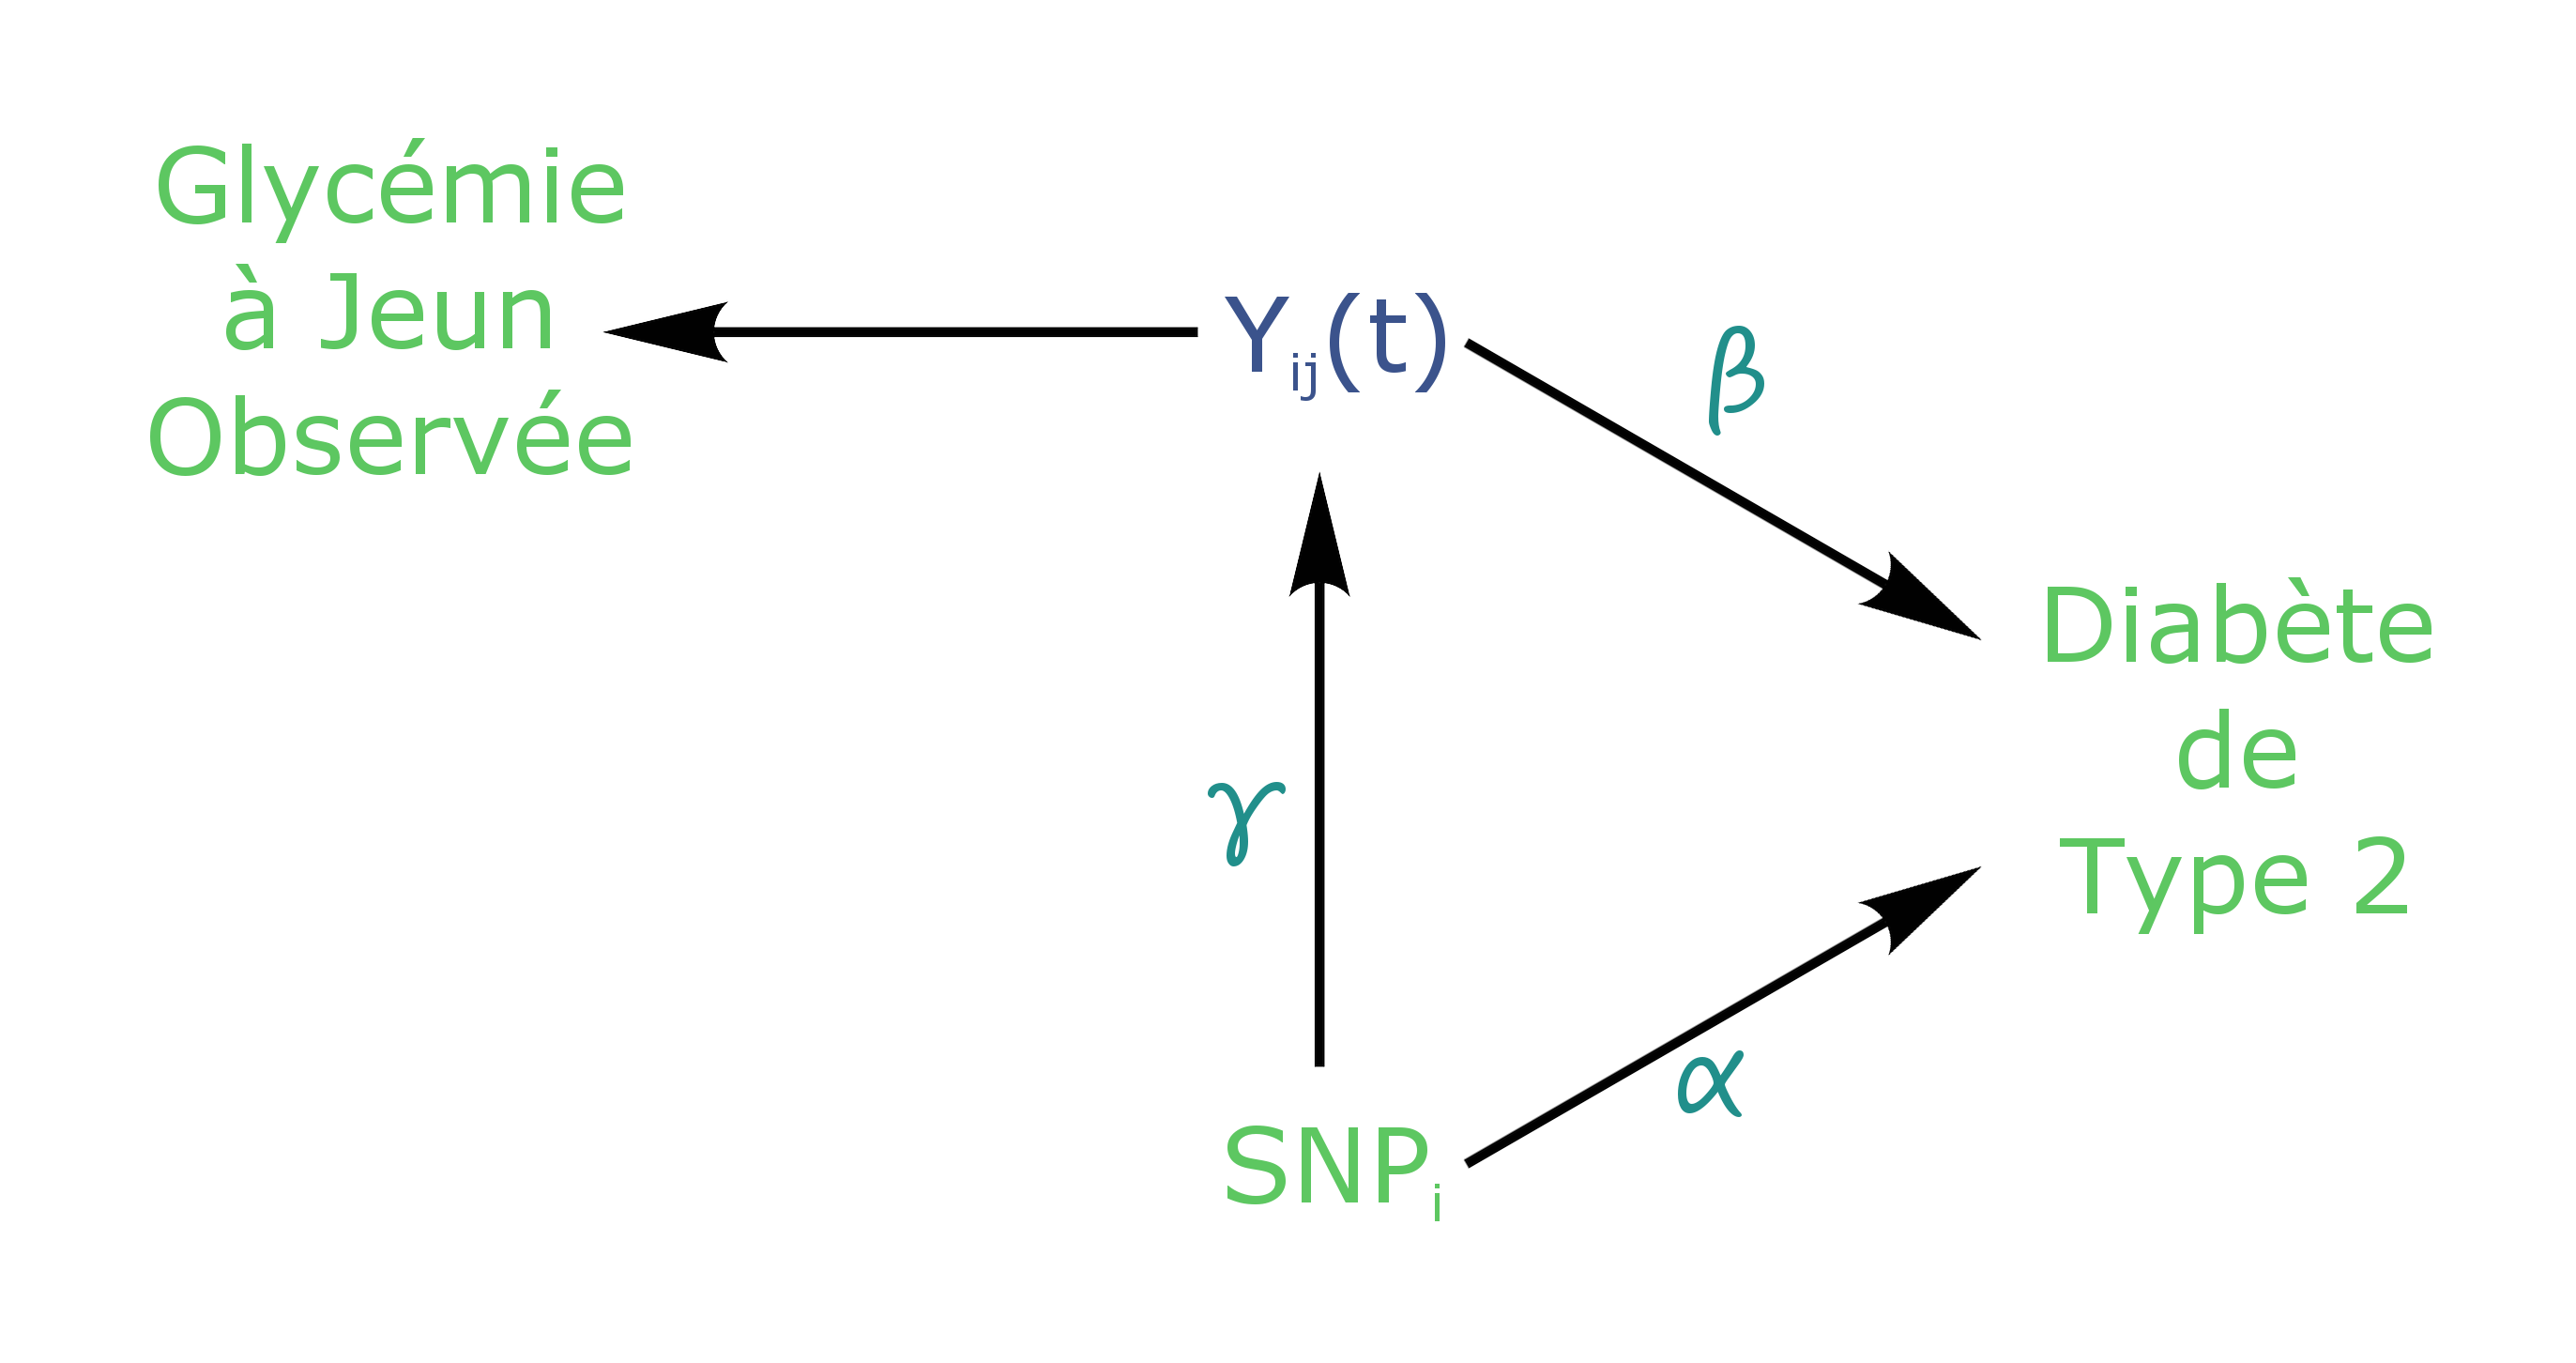
\includegraphics[width=0.90\linewidth]{jointModel.png}}
    \captionof{figure}{\color{springgreen3} Diagramme causal du Modèle Joint (adaptée de \mbox{\citet{ibrahim2010}}).}
    \label{Fig1}
\end{center}
% \vspace{2cm}
\par{La composante longitudinale consiste généralement en un modèle (linéaire) mixte:}

\begin{minipage}[t]{0.475\columnwidth}
\vspace{-1cm}%
\hspace{-10cm}
{\color{springgreen3}%
\begin{eqnarray}Y_{ij}(t_{ij})=X_{ij}(t_{ij})+\epsilon_{ij}\nonumber\label{Eq1}\end{eqnarray}
\begin{eqnarray}X_{ij}(t_{ij})=\theta_{0i}+\theta_{1i}t_{ij}+\gamma SNP_i\nonumber\label{Eq2}\end{eqnarray}
\begin{eqnarray}\boldsymbol\theta \sim \mathcal{N}_2(\boldsymbol\mu, \boldsymbol\Sigma)\nonumber\label{Eq3}; \epsilon_{ij} \sim \mathcal{N}(0, \sigma^2)\nonumber\label{Eq4}\end{eqnarray}
}%
\vspace{-1cm}
\end{minipage}%
\hfill\vline\hfill
\begin{minipage}[t]{0.475\columnwidth}%
\vspace{0.8cm}%
\par{{\color{springgreen3}$Y_{ij}(t_{ij})$}: valeur observée;}
\vspace{0.25cm}%
\par{{\color{springgreen3}$X_{ij}(t_{ij})$}: valeur vraie (non observée) de la variable longitudinale;}
\vspace{0.25cm}%
\par{{\color{springgreen3}$\gamma$}: effet du SNP sur la trajectoire (\mbox{\bref{Fig1}{Figure}}).}
\end{minipage}
\vspace{3cm}
\par{Un modèle de Cox (risque proportionnel) pour la composante de survie (incidence):}
{\color{springgreen3}\begin{eqnarray}\lambda_i(t_{ij})=\lambda_0(t_{ij}) exp(\beta X_{ij}(t_{ij})+\alpha SNP_i)\nonumber\label{Eq5}\end{eqnarray}}
\begin{minipage}[t]{0.475\columnwidth}
\vspace{0.10cm}%
\par{{\color{springgreen3}$\lambda_i(t_{ij})$}: fonction de risque au temps {\color{springgreen3}$t_{ij}$}}
\vspace{1.85cm}%
\par{{\color{springgreen3}$\lambda_0(t_{ij})$}: fonction de risque de base (non spécifiée).}
\end{minipage}%
\hfill\vline\hfill
\begin{minipage}[t]{0.475\columnwidth}%
\vspace{0.10cm}%
\par{{\color{springgreen3}$\alpha$}: effet du SNP sur le temps de survenue de l'événement (\mbox{\bref{Fig1}{Figure}}).}
\par{{\color{springgreen3}$\beta$}: lien entre la trajectoire et le temps de survenue de l'événement (\mbox{\bref{Fig1}{Figure}}).}
\end{minipage}


%----------------------------------------------------------------------------------------
%    RESULTS
%----------------------------------------------------------------------------------------
\section*{Données: \large{La Cohorte D.E.S.I.R.}}
\vspace{-1.5cm}
\par{\mbox{4 352} individus (167 DT2 incident) de la cohorte D.E.S.I.R. et \mbox{101 165} SNPs (Illumina Metabochip) ont été analysés par un modèle joint (\cmd{JM}\ \citep{rizopoulos_jm_2010}).
La puissance statistique a été également étudiée pour comparer le modèle joint aux approches transversales classiques (régression linéaire et logistique).}

\section*{Résultats: \large{Modèle Joint et Metabochip}}
\vspace{-0.5cm}
\begin{center}
    \fbox{\includegraphics[width=0.9\linewidth]{/disks/DATA/DESIR_longitudinal/Article/SFD2017/JointModel_EstimationsGWAS.pdf}}
    \captionof{figure}{\textcolor{springgreen3}{SNPs nominalement associés ($\textrm{p-valeur}<0,05$) à l'incidence de DT2 et la glycémie à jeun (265 variants / 161 gènes uniques).}}
    \label{Fig2}
\end{center}
\vspace{1cm}
\begin{center}
    \large{\input{"/disks/DATA/DESIR_longitudinal/Article/SFD2017/SFD2017_Table1.tex"}}
    \captionof{table}{\textcolor{springgreen3}{Estimation par modèle joint (\cmd{JM} \citep{rizopoulos_jm_2010}).}}
    \label{Tab1}
\end{center}
\vspace{1cm}
\begin{center}
    \fbox{\includegraphics[width=0.9\linewidth]{/disks/DATA/DESIR_longitudinal/Article/SFD2017/CMvJM.pdf}}
    \captionof{figure}{\textcolor{springgreen3}{Puissance et Erreur de Type 1 de 265 SNPs (\mbox{\bref{Fig2}{Figure}})}}
    \label{Fig3}
\end{center}


%----------------------------------------------------------------------------------------
%    FUTURE RESEARCH
%----------------------------------------------------------------------------------------
\section*{Conclusion}
\vspace{-1cm}
\begin{itemize}
\item Puissance statistique supérieure via l'approche par Modèle Joint (\mbox{\bref{Fig3}{Figure}}), comparée aux approches classiques (régression linéaire et logistique).
\vspace{0.5cm}
\item SNPs montrant un effet simultané sur la glycémie et le risque de DT2 (p.ex. \textcolor{maroon2}{TCF7L2}, \mbox{\bref{Fig2}{Figure}}).
\vspace{0.5cm}
\item rs10830963\_G (\textcolor{maroon2}{MTNR1B}) montre des effets contre-intuitifs entre une augmentation de la glycémie (\textcolor{springgreen3}{$\gamma$}) et une baisse du risque de DT2 (\textcolor{springgreen3}{$\alpha$}) dans D.E.S.I.R. (\mbox{\bref{Tab1}{Table}}).
\end{itemize}


\end{multicols}
%----------------------------------------------------------------------------------------
%    REFERENCES
%----------------------------------------------------------------------------------------
\color{SaddleBrown}
\small
\bibliographystyle{apalike} % apalike
\bibliography{SFD2017.bib} % Use the example bibliography file sample.bib
\begin{center}
    \vfill
    {
\includegraphics[height=5.5cm, keepaspectratio]{../UTILS/Logos/logo_cnrs.pdf}
    \hspace{11cm} 
\includegraphics[height=5.5cm, keepaspectratio]{../UTILS/Logos/UL2-WEB-2014.png}
    \hspace{8cm} 
\includegraphics[height=5.5cm, keepaspectratio]{../UTILS/Logos/Institut-Pasteur-de-Lille.png}
    \hspace{11cm} 
\includegraphics[height=5.5cm, keepaspectratio]{../UTILS/Logos/logo_egid.pdf}}
\end{center}


%----------------------------------------------------------------------------------------
\end{document}